%!TEX root = ../template.tex
%%%%%%%%%%%%%%%%%%%%%%%%%%%%%%%%%%%%%%%%%%%%%%%%%%%%%%%%%%%%%%%%%%%%
%% chapter4.tex
%% NOVA thesis document file
%%
%% Chapter with lots of dummy text
%%%%%%%%%%%%%%%%%%%%%%%%%%%%%%%%%%%%%%%%%%%%%%%%%%%%%%%%%%%%%%%%%%%%

\typeout{NT FILE chapter4.tex}%

\chapter{Implementation}
\label{cha:implementation}

\section{Architecture} % (fold)
\label{sec:architecture}
The system was built using a modular approach,
each module is entirely self-contained, making it simple to expand or replace system functionality.
The system components are split into two distinct areas: runtime, and pipeline components.
The runtime comprises all essential components to the system liveliness,
whereas the pipeline covers all components needed during the system's provisioning and development.

\subsection{Runtime Architecture} % (fold)
\label{sec:runtime_architecture}

The only novel component introduced in a typical microservices runtime environment is the proxy adapter.
An example with three microservices is depicted in Figure~\ref{fig:runtime}.
In this example, the Account's microservice has undergone three major API changes.
The Inventory microservice, which is dependent on the previous service, has been updated to reflect the changes, but the Shipping microservice has not been updated and is two versions behind.

\begin{figure}[htbp]
    \centering
    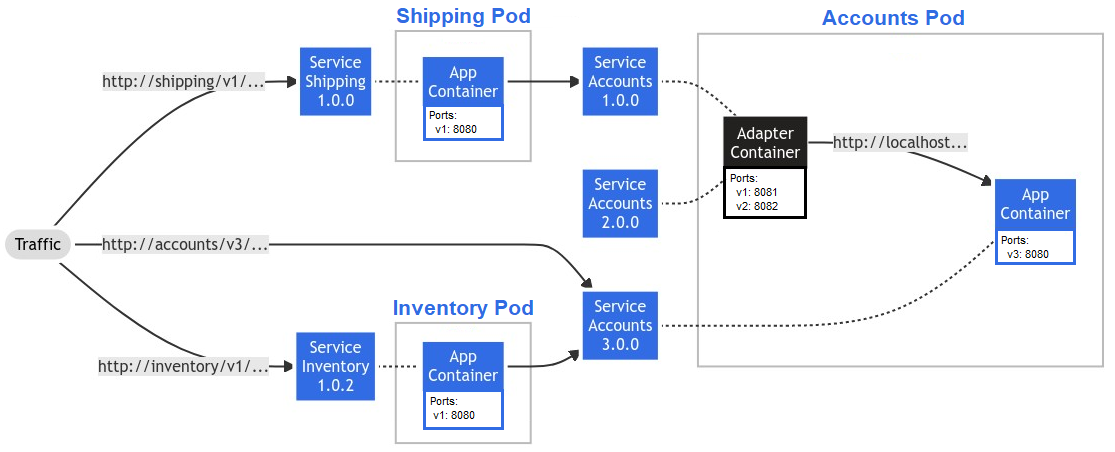
\includegraphics[height=2.4in]{runtime}
    \caption{Example of a runtime configuration}
    \label{fig:runtime}
\end{figure}

Every contract version that is still in use has its own unique K8s service, as can be seen for the three versions of the Accounts microservice.
Older versions are supported by the adapter, while the most up to date version is directly supported by the microservice app.
A consumer accesses a producer app via the service that has the same version as the one specified in its code.

Containers are selected in services policies by attributing names to their exposed ports and assigning the same name on the target port of the service policy.
In adapter containers, one port is exposed for each of the supported contract versions and named with the version number.

When a microservice app is upgraded via a rolling update,
the services never become unavailable:
they point either to the adapter containers or the application containers, depending on whether the affected pods finished the upgrade process.
In the traditional approach all consumers would need to be upgraded in tandem with their consumed services in order to avoid downtime.

\subsection{DevOps Pipeline} % (fold)
\label{sec:devops_pipeline_architecture}

A proof-of-concept pipeline was developed, its architecture is depicted in Figure \ref{fig:pipeline}.
The nodes depicted in blue represent the introduced novel stages.
If a service only underwent changes that did not affect its API or dependencies, the introduced stages are skipped.

\begin{figure}[htbp]
    \centering
    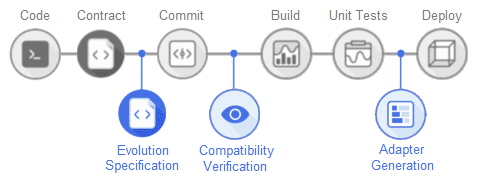
\includegraphics[height=1.5in]{pipeArch}
    \caption{DevOps Pipeline}
    \label{fig:pipeline}
\end{figure}

The pipeline was developed using the Jenkins~\cite{jenkins} pipeline suite, each of the novel stages is supported by a distinct Java application that is pulled from version control
and executed directly on the pipeline, whereas the other stages are supported natively by the suite.
The modules that enable each novel stage will be discussed in detail in the following sections.

\section{Contract Representation} % (fold)
\label{sec:contract_representation}

The OpenAPI specification is the most
widely adopted WADL for HTTP services, instead of designing yet another WADL, it was
adopted the OpenAPI specification to support the needs of the implementation.
Designing a WADL tailored for this problem would be counterproductive because teams rely on other tools,
and supporting an additional WADL would require the development of an extensive converter tool
that would need to be constantly maintained in order to support changes in new versions of the OpenApi and the new WADL specification's.

To represent records in messages, it was chosen the JSON format, because of its simplicity and widespread adoption.
There are more performant formats that have a binary representation,
however such formats are typically not supported by front-end frameworks, and for the purpose of this prototype
it is not important to measure the performance of different object serialization protocols, since
there are already sources that provide comparisons in this regard between XML, JSON, Protobuf, Thrift and other popular formats \cite{serializationBenchmark}.

The schema of JSON records must be described.
The OpenAPI standard includes a schema description language in its Web API description language, that supports JSON records.
There are dedicated JSON schema description languages (such as the JSON-schema project \cite{jsonschema}), however,
using a language other than OpenApi, would necessitate decoupling the specification of schemas from the specification of HTTP endpoints.
This would require additional effort on the part of the developing team to maintain the cross-references
between each specification manifest, and their versions.

A snippet of a \textit{Pet Store} OpenApi contract can be seen in Figure \ref{fig:open_contract}.
In this example we can view the specification of a JSON schema for a Pet data object,
as well the specification for an HTTP endpoint.
OpenApi allows properties to be defined robustly with specification of not only their type but also their format, as shown in line 31.

The types and formats of properties are standardized between object schemas and HTTP parameters.
Properties have the following data types: string, number, integer, boolean, array, and object.
Property formats are free-form, yet there are established conventions for the most commonly used formats.

The current implementation only supports services with a RESTFul API.
Advanced OpenAPI specification features such as parameters with alternative types are not supported (e.g Type:=OneOf(String, Integer)).

\begin{figure}[htbp]
    \centering
    \centerline{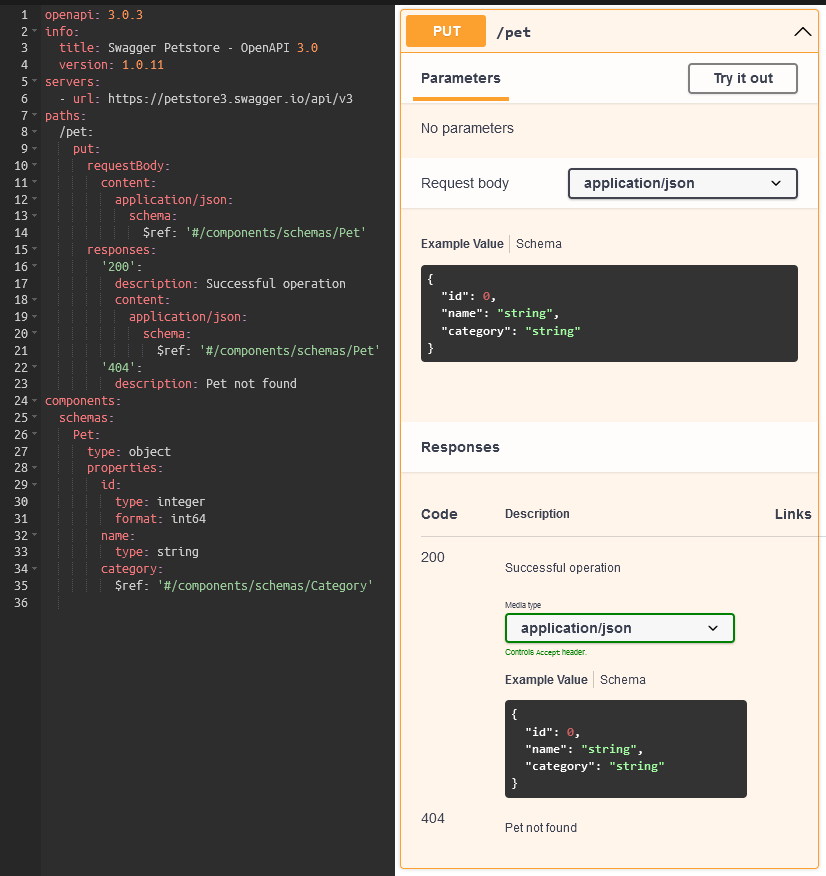
\includegraphics[height=6.5in]{openContract}}
    \caption{OpenAPI contract example}
    \label{fig:open_contract}
\end{figure}

\newpage

The specification of the dependencies of a service was done using Helm \cite{helm}.
Helm is package manager for Kubernetes that allows developers to more easily package, configure, and deploy applications and services onto Kubernetes clusters.
A chart is a Helm package, composed of a collection of files that describe a related set of Kubernetes resources.
The most significant components of a Chart are the:
\begin{itemize}
    \item The Chart.yaml, that allows the definition of the Chart dependencies and other meta-information about the application such as its name and version;
    \item The Template's directory, that contains incomplete Kubernetes manifests \textit{Templates} such as Services, Deployments, DaemonSets, Namespaces and so on;
    \item The Values.yaml, that contains key-value pairs used to complete the definition of each template. Values can be overridden when the chart is deployed, the file is used to define the default values.
\end{itemize}
A single chart might be used to deploy something simple, like a single Kubernetes pod, or something complex, like a complete web app stack with HTTP servers, databases, caches, and so on.
The typical approach is to define an individual chart for each distinct microservice, so that they can be upgraded individually.
If a single chart is used to deploy multiple services it is no longer possible to represent accurately the dependencies of each service
in the chart definition, because the chart syntax doesn't allow the individual definition of the dependencies of each service, it only allows the declaration of the dependencies of the deployment as a whole.

An example of the definition of a service/chart dependencies can be seen in Listing \ref{lst:helm}.
The dependencies of a service are mapped indirectly, each dependency point to a Helm chart that is implicitly associated with one service.

\begin{lstlisting}[caption=Chart.yaml example, label=lst:helm, captionpos=b]
dependencies:
    - name: nginx
      version: "1.2.3"
      repositiry: https://example.com/charts
    - name: memcached
      version: "3.2.1"
      repositiry: https://another.example.com/charts
\end{lstlisting}

The declaration of resources consumed by a service is defined in chart template files.
For each deployment template it was defined the resources consumed by its containers by
setting the minimum amount of CPU and Memory resources (represented on the requests key) and by setting a limit on these resources (represented on the limits key).
An example of the definition of a service resources can be seen in Listing \ref{lst:resource}.

\begin{lstlisting}[caption=Helm template resources example, label=lst:resource, captionpos=b]
apiVersion: v1
kind: Pod
sepc:
    containers:
    - name: app
      image: images.my-company.example/app:v4
      resouces:
        request:
          memory: "64Mi"
          cpu: "250m"
        limits:
          memory: "128Mi"
          cpu: "500m"
\end{lstlisting}

\section{Contract Interpretation} % (fold)
\label{sec:contract_interpretation}

The interpretation of a contract specification is done in a dedicated module named ''Parser''.
This module is meant to be used as Java library by other modules,
it interprets contracts written in OpenApi format and provides a read-only Java interface
that is agnostic to the original specification format.

The implementation of the parser module uses the Swagger-parser project \cite{swaggerparser} to convert OpenApi contracts into a Java POJO representation.
The OpenApi POJO representation is accessed through a custom read-only wrapper class and interface.
All the forthcoming modules operate under this interface instead of the OpenApi POJO format.

Although it was adopted the OpenApi format the solution is not dependent on it, as the parser module provides a decoupling point.
This enables the specification of different contract to be written in different or even mixed WADL,
as long as the parser module is extended to support the new WADL's.
The interpretation of service resources and dependencies written in Helm charts is also supported by the parser module under a separate interface.

\section{Evolution Representation} % (fold)
\label{sec:evolution_representation}

The evolution of contracts is represented in a custom description language.
The description only maps the details about the changed procedures of a service,
it is not necessary to map the changes in service dependencies and resource requirements because they can be inferred by comparing the last two contract versions.
The description language haves the following format:

\begin{itemize}
    \setlength\itemsep{0em}
    \item \textbf{Procedures:} List of the procedures that are adapted between contract versions.
    \begin{itemize}
        \setlength\itemsep{0em}
        \item \textbf{Endpoint:} The endpoint of the procedure and its HTTP method in the new contract.
        \item \textbf{Prior Endpoint:} The endpoint of the procedure and its HTTP method in the previous contract.
        \item \textbf{Messages:}  List of the messages exchanged by the procedure in the new contract version (the request message and response messages).
        \begin{itemize}
            \setlength\itemsep{0em}
            \item \textbf{Type:} The response or request type in the new contract. \\\textit{(e.g. REQUEST, 200, 400, etc)}
            \item \textbf{Prior Type:} The response or request type in the previous contract.
            \item \textbf{Parameters:} List of the parameters of the message (Path, Query, Header, Cookie and Body parameters).
            \begin{itemize}
                \setlength\itemsep{0em}
                \item \textbf{Key:}  The identifier of the parameter. \\\textit{(e.g path|quantity)}
                \item \textbf{Resolution:} The specification of a resolution for a parameter. \\\textit{(eg. link=query|limit)}.
                \item \textbf{Type:} The type of the parameter. \\\textit{(eg. String)}
                \item \textbf{Format:} The format of the parameter. \\\textit{(eg. yyyy-mm-dd hh:mm:ss)}
            \end{itemize}
        \end{itemize}
    \end{itemize}
\end{itemize}

The first segment of parameter keys represents the parameter location (e.g.Path, Query, Header, Cookie and Body parameters), the second segment represents the ''name'' of the parameter.
\[ \langle location\rangle |\langle name\rangle \;\;\;(e.g\;path|quantity) \]
Schemas used in a message body are flattened into multiple parameters:
\[ \mathbf{Item}\bm{\{}id,price\bm{\}} \rightarrow json|item.id,\;json|item.price \]
The schema Item is flattened into two distinct parameters, which are mapped by specifying the hierarchy path in the parameter name.

As previously mentioned in Section \ref{sec:evolution_specification}, resolutions can have one of three distinct types DefaultValue, Link or Function.
The type of resolution is represented in the first segment of a resolution rule, while the second segment represents the resolution itself:

\begin{itemize}
    \item \textbf{Default value resolution:} \[ default=\langle value\rangle \;\;\;(e.g\;default=true) \]
    \item \textbf{Link resolution:} \[ link=\langle location\rangle|\langle name\rangle \;\;\;(e.g\;link=query|limit) \]
    \item \textbf{Function resolution:} \[ function=\langle expression\rangle \;\;\;(e.g\;function=json|name + json|surname) \]
\end{itemize}

Function resolutions are written as one line Java expressions that can use parameters of the previous contract. The
parameters are referenced by their location and name.

The description language supports arrays in request and response schemas.
Arrays are defined by bracketing the array elements of a parameter.
\[ \mathbf{Item}\bm{\{}tags:Tag[]\bm{\}}\;\;\;\mathbf{Tag}\bm{\{}id:String\bm{\}} \rightarrow \;json|item.[tags].id \]
\[ \mathbf{Item}\bm{\{}tags:Tag[]\bm{\}}\;\;\;\mathbf{Tag}\bm{\{}keywords:String[]\bm{\}} \rightarrow \;json|item.[tags].[keywords] \]
Link resolution's between two parameters with the same number of array elements are resolved by matching the members of the different array elements.
If a Link resolution uses parameters with a different number of array elements, the first members of the unpaired array elements are selected, while remaining array members are ignored.

The Listing \ref{lst:evolution_example} depicts an example of a evolution description in this language.

\begin{lstlisting}[caption=Evolution specification example, label=lst:evolution_example, captionpos=b]
procedures:
- endpoint: /pets GET
  endpoitPrior: /pets GET
  messages:
  - type: Request
    typePrior: Request
    parameters:
    - key: query|limit
      resolution: link=path|limit
      type: String
      format: none
  - type: '200'
    typePrior: '200'
    parameters:
    - key: json|[pet].name
      resolution: function=json|[pet].first_name + [pet].surname
      type: String
      format: none
    - key: json|[pet].birth
      resolution: function=LocalDate.now().getYear() - json|[pet].age
      type: String
      format: yyyy
\end{lstlisting}

To minimize the documentation effort it was developed a GUI editor that facilitates the specification of evolutions.
Figures \ref{fig:editor1} and \ref{fig:editor2} depict the editor interfaces.
The editor was implemented as an IDE Plugin, the current implementation supports the IntelliJ integrated development environment.

\begin{figure}[htbp]
    \centering
    \centerline{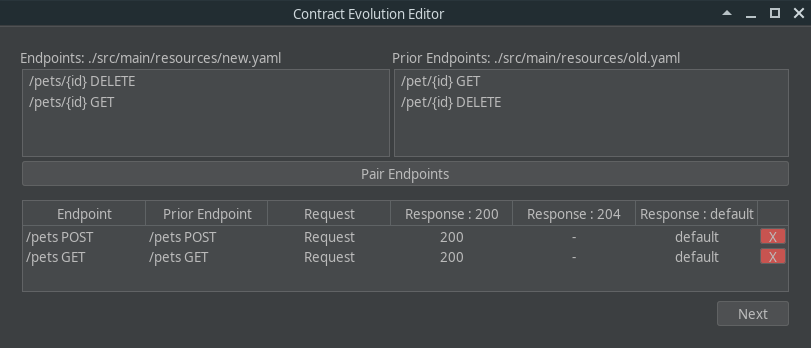
\includegraphics[height=2.6in]{editor2}}
    \caption{Evolution editor, procedure mappings}
    \label{fig:editor1}
\end{figure}

\begin{figure}[htbp]
    \centering
    \centerline{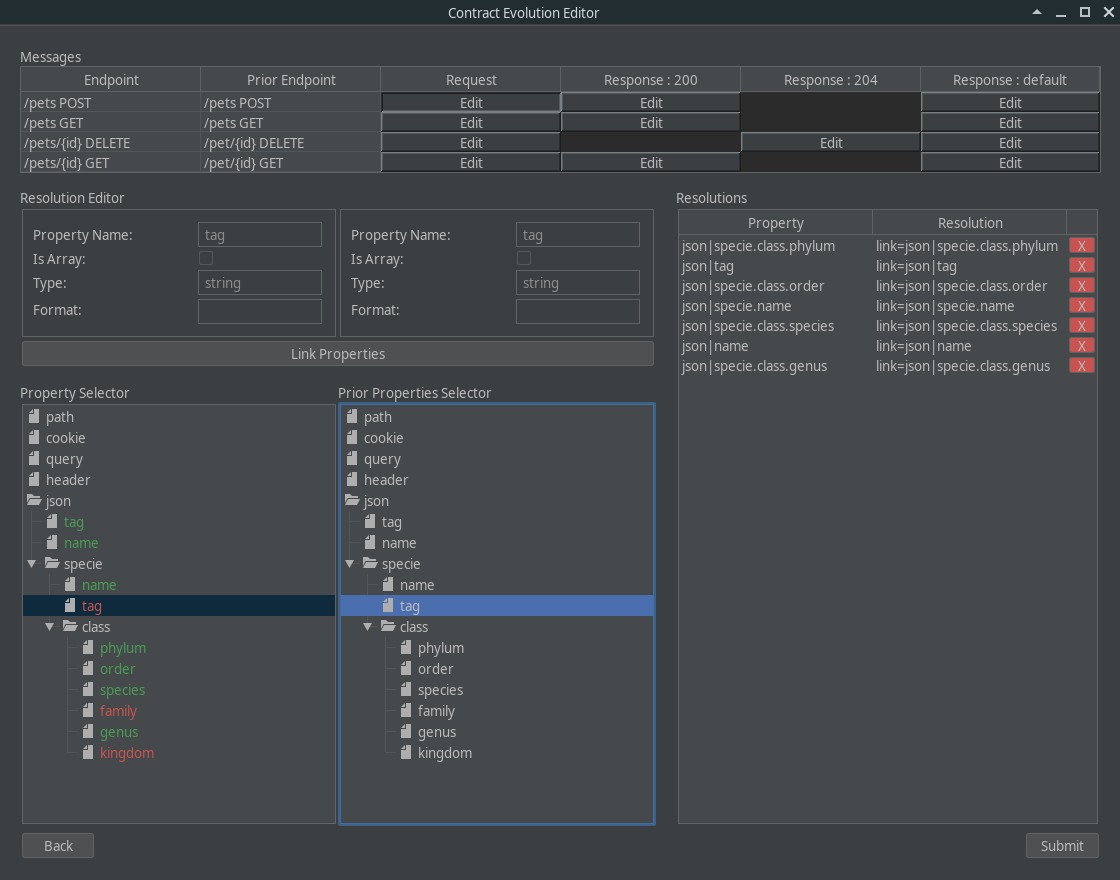
\includegraphics[height=4.6in]{editor1}}
    \caption{Evolution editor, parameter mappings}
    \label{fig:editor2}
\end{figure}

The editor compares two contract versions,
and automatically maps all the elements that haven't changed from one version to the other, the
developer is left with the task of explicitly mapping the remaining elements.

The editor starts by requesting the developer to map endpoints in the new contract to endpoints in the old contract,
afterwards the developer must match each of the endpoint messages and specify a resolution for all the parameters that changed
in a contract, unresolved parameters are highlighted in red.

The right column of the editor~\ref{fig:editor2} holds the resolutions that were already mapped.
The uppermost left column allows the developer to write rules for each unresolved parameter.
The developer can select leaf parameters in the hierarchy, or choose intermediate parameters.
If they choose an intermediate parameter and input a resolution rule, then all child parameters are also resolved.

After all parameters are resolved the developer submits the resolutions, and
the editor outputs an evolution specification file with the same description language presented in the beginning of this section.

\section{Compatibility Verification} % (fold)
\label{sec:compatibility_verification}

The compatibility verification process is done by a dedicated module named ''Verifier''.
This module was implemented in Java as a command-line application.
The module verifies if the provided evolution specification is valid.
In Algorithm \ref{alg:evoalg} it is presented the pseudo-code of the compatibility verification process.
It starts by checking if all the procedures and messages of prior contract are present in the specification,
then it verifies the validity of the resolutions for each parameter of the new contract messages.
\begin{itemize}
    \setlength\itemsep{0em}
    \item [Resolutions can be invalid due to four reasons:]
    \item Invalid syntax in resolution expressions;
    \item References parameters that don't exist in the previous contract;
    \item Uses functions that are not supported;
    \item Uses resolutions that have a different type and format then the parameter.
\end{itemize}

The present implementation of the verifier module does not check whether the cluster has adequate computational resources to provision the service or whether all service dependencies are alive and reachable.
These functionalities were not implemented since the Helm deployment process already performs these verifications prior to the deployment of a service.
Nonetheless, including these verifications in the verifier module could be useful in order for the solution to be decoupled from Helm.

The module also does not verify if the type and format of a function resolution matches the type and format of a parameter.
To support this validations in verifier module with would be necessary to use a dedicated language for specifying function resolutions.
The verification of correct function resolution types is done alternatively by the generator module that verifies compile-time errors when parameter references are substituted by real values.

\begin{algorithm}
    \caption{Evolution validation algorithm}\label{alg:evoalg}
    \begin{algorithmic}[1]
        \Procedure {ValidateEvolution}{$Evolution$, $PriorContract$, $NewContract$}
            \State \textbf{assert} $PriorContract.procedures \subseteq Evolution.procedures\rightarrow priorEndpoint$
            \ForAll {$pd \in Evolution.procedures$}
                \State \textbf{assert} $pd \in NewContract.procedures$
                \State $PriorMessages \leftarrow PriorContract.getMessages(pd.priorEndpoint)$
                \State $NewMessages \leftarrow NewContract.getMessages(pd.endpoint)$
                \State \textbf{assert} $PriorMessages \subseteq pd.messages$
                \ForAll {$msg \in pd.messages$}
                    \State \textbf{assert} $msg \in NewMessages$
                    \State \textbf{assert} $msg.parameters = NewMessages.get(msg).parameters$
                    \ForAll {$prm \in msg.parameters$}
                        \State $OldMessage \leftarrow PriorMessages.get(msg.priorType)$
                        \State \textbf{assert} $VerifyResolution(prm, OldMessage)$
                    \EndFor
                \EndFor
            \EndFor
        \EndProcedure
        \Statex
        \Procedure {VerifyResolution}{$Parameter$, $OldMessage$}
            \State $Resolution \leftarrow Parameter.resolution$
            \If {$Resolution.type = Value$}
                \State \textbf{assert} $Resolution.value\ \textbf{instanceof}\ Parameter.type$
                \State \textbf{assert} $format(Resolution.value) = Parameter.format$
            \ElsIf {$Resolution.type = Link$}
                \State \textbf{assert} $Resolution.parameter \in OldMessage.parameters$
                \State \textbf{assert} $Resolution.parameter.type = Parameter.type$
                \State \textbf{assert} $Resolution.parameter.format = Parameter.format$
            \ElsIf {$Resolution.type = Function$}
                \State \st{\textbf{assert} $Resolution.function.returnType = Parameter.type$}
                \State \st{\textbf{assert} $Resolution.function.returnFormat = Parameter.format$}
                \ForAll {$prm \in Resolution.function.parameters$}
                    \If {$prm.key == null\;\&\&\;prm.resolution != null$}
                        \State \textbf{assert} $VerifyResolution(prm, OldMessage)$
                    \Else
                        \State \textbf{assert} $prm \in OldMessage.parameters$
                    \EndIf
                \EndFor
            \EndIf
        \EndProcedure
    \end{algorithmic}
\end{algorithm}

\section{Adapter Generation} % (fold)
\label{sec:adapter_generation}

The generation of the proxy adapter code is done in a dedicated module named ''Generator''.
The adapter is generated by populating a template implementation with the information provided in evolution specifications.
The adapter must be able to support all prior versions that are still in use, and adapt them to the last contract version.

Evolution specifications only provide information on how to adapt messages from contiguous versions (eg. v1\textrightarrow v2).
The information necessary to adapt messages from discontinuous versions is obtained by chaining the evolution specifications and
merging their resolutions. Figure \ref{fig:merge} exemplifies the merge process.

\begin{figure}[htbp]
    \centering
    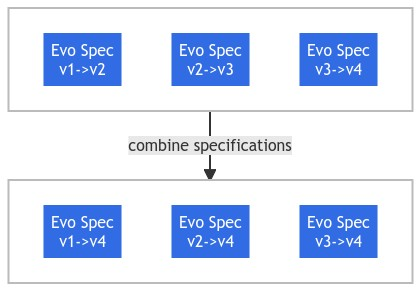
\includegraphics[height=2in]{merge}
    \caption{Evolution specification merge process example}
    \label{fig:merge}
\end{figure}

This module begins by querying the active versions of the target service with the Kubectl command-line tool.
Kubectl~\cite{kubectl} is a tool that interfaces with Kubernetes clusters and can be used to inspect and manage cluster resources.

After determining the active service versions, this module retrieves all evolution specifications up to the oldest version that is still active,
and then combines them so that all specifications link to the current version.

Link resolution rules can be chained together in a straightforward manner.
Function resolutions are chained together by recursively replacing missing parameter references with their resolutions .
Below in Table~\ref{table:1} it is presented an example, where resolution rules are chained incrementally from the two last versions to the oldest version:

\begin{table}[h!]
\centering
\begin{tabular}{|l|l|l|}
    \hline
    \thead{Transition} &  \thead{Missing^*} & \thead{Resolution for parameter := path|seven_7} \\
    \hline
    v_3\rightarrow v_4 & 7 & function=path|five_5 + path|two_2  \\    \hline
    v_2\rightarrow v_4 & 7,2 & function=path|five_5 + (default=2)_2  \\    \hline
    v_1\rightarrow v_4 & 7,5,2 & function=(function=path|three_3 + (default=2)_2)_5 + (default=2)_2 \\    \hline
\end{tabular}
\begin{tablenotes}
    \flushleft
    \tiny
    *Indicates the missing parameters in the prior contract (e.g 7\textlangle =\textrangle path|seven)
\end{tablenotes}
\caption{Chained resolution rules example}
\label{table:1}
\end{table}



\section{Adapter} % (fold)
\label{sec:adapter}

The adaption approach consists on: for each endpoint the
adapter re-constructs the entire request from zero and populates the parameter resolutions with the information of the original request.
The adapter server exposes each of the supported contract version's in a distinct port.
A Kubernetes service is created for accessing each of the adapter ports.

The Function resolutions are written as one-line Java expressions.
The resolutions are injected directly into the template implementation of the adapter, and the parameter references in the resolution are then replaced with the parameters themselves.
The adapter's current template implementation does not support HTTPS, however this can be added.
Because TLS is mandatory in HTTP 1.2, the implementation only supports HTTP 1.1.

The adapter was built with Spring Boot and an Apache Tomcat/9.0.65 HTTP server, the base image of the adapter docker container is an "openjdk:11-nanoserver".
In order to prevent the JVM from calling garbage collector frequently and reallocating the heap memory while Tomcat is trying to serve requests,
the JVM has started with a higher maximum heap memory, and the initial heap memory
size was set to the same value as its maximum memory size.
The minimum and maximum number of threads for Tomcat was set to 15 and 2000 respectively, in order to support a higher load of requests.

TODO pseudo codigo

